\section{Ceph Evaluation: Initial Results and Tunings}
\label{sec:ceph-initial}

\subsection{Ceph RADOS Scaling}


RADOS is a reliable distributed object store, the foundational component for
CephFS file system. There are two types of scaling tests we are interested at
the RADOS layer:

\begin{itemize}
  \item scaling on the number of OSD servers
  \item scaling on the number of OSDs per OSD server
\end{itemize}

Our system setup poses some limitations on the scalability tests we wanted to
perform. In particular, we currently had four OSD servers, eight clients, and
eleven OSD servers per client. The scaling tests, therefore, will be within
these constraints.

We used the open-source RADOS Bench tool, developed by Inktank, to perform our
initial performance analysis of the underlying RADOS layer.  RADOS Bench simply
writes out objects to the underlying object storage as fast as possible, and
then later reads those objects in the same order as they were written.

\subsubsection{Disable TCP autotuning}

\begin{figure}[htb]
\centering
%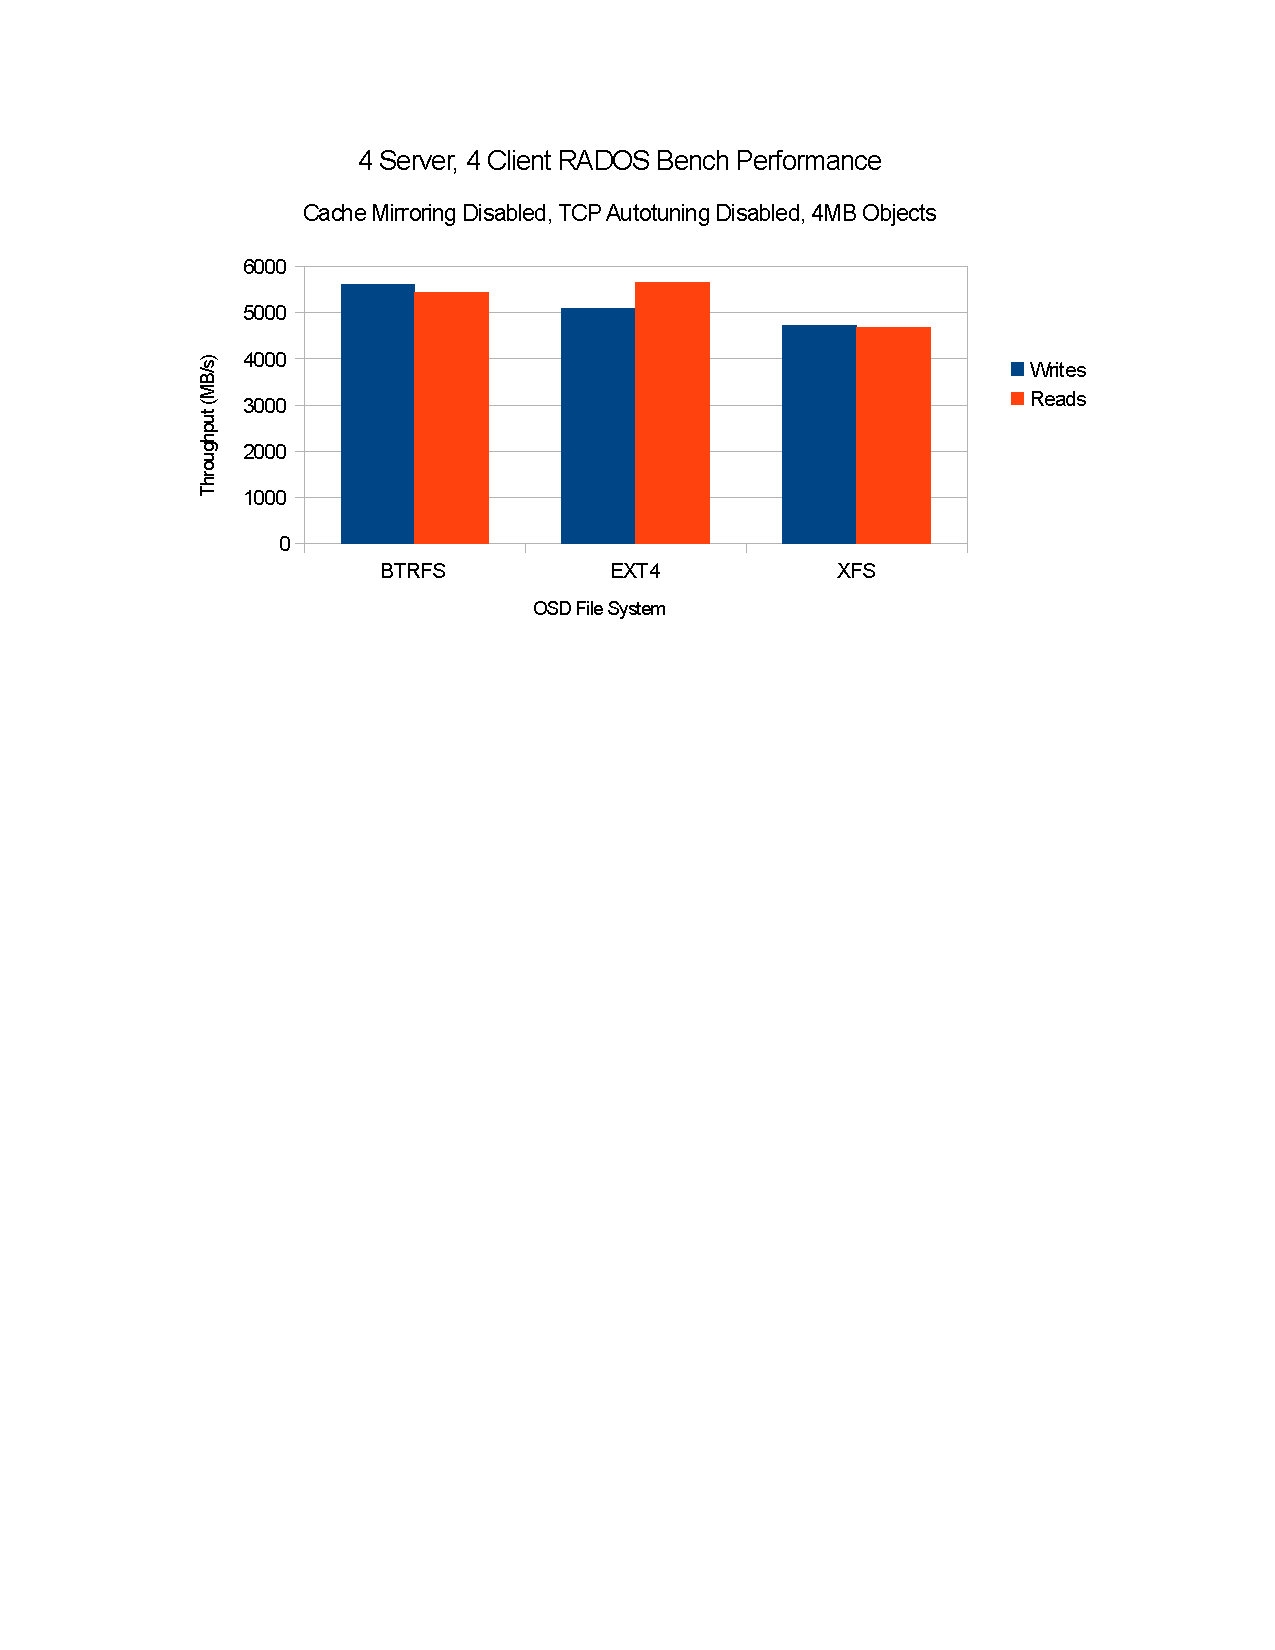
\includegraphics[width=3.5in]{rados-after-ddn-tcptune}
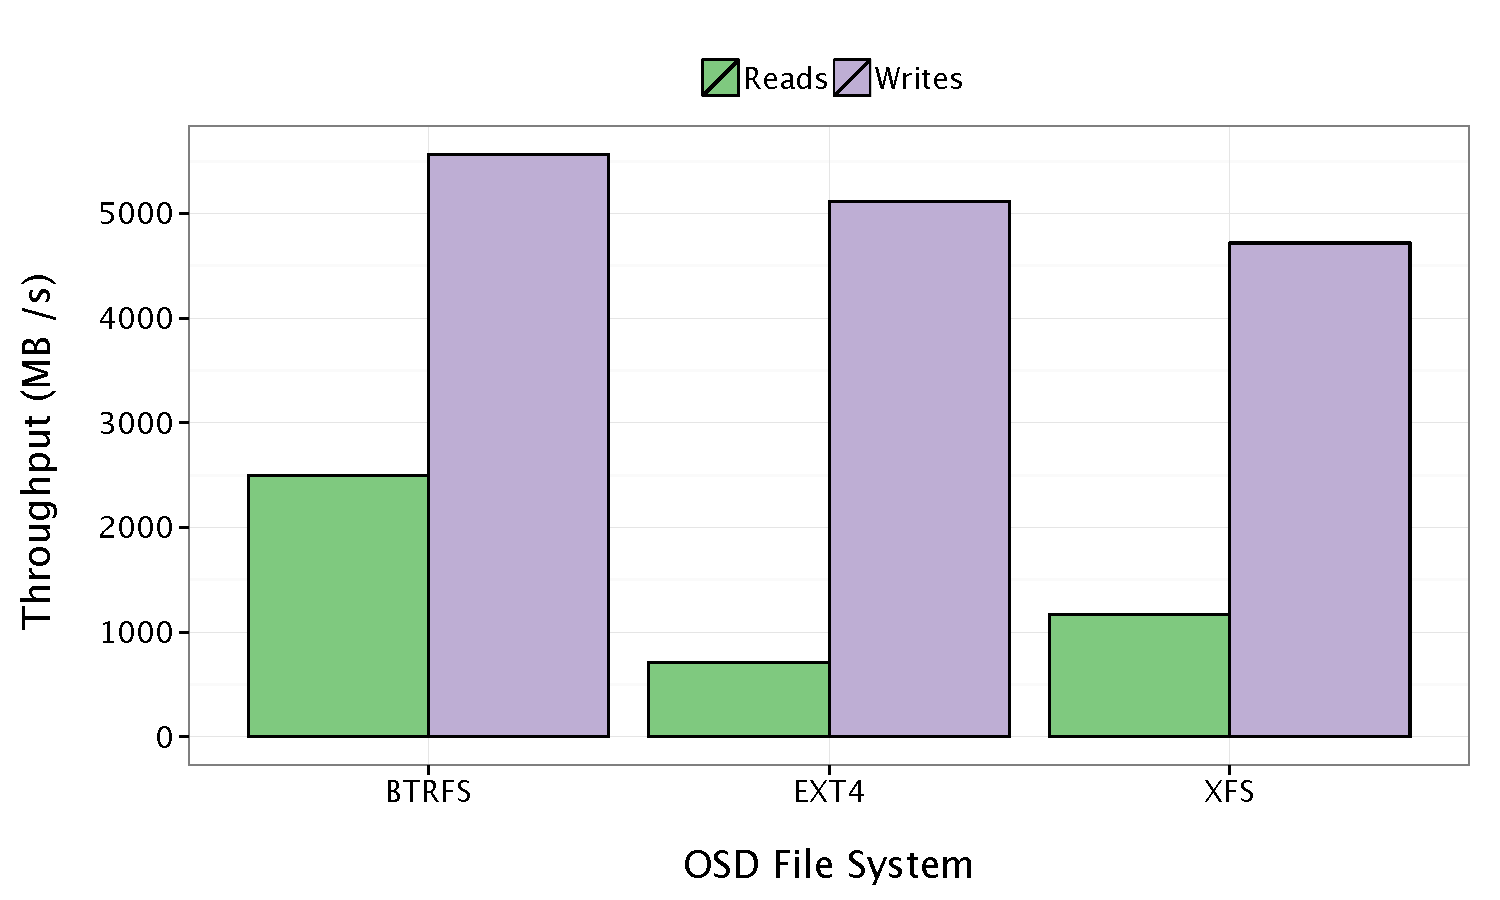
\includegraphics[width=3.5in]{autotune-enabled}
\caption{Evaluating RADOS bench \textbf{with} TCP auto tuning, 4 servers, 4
clients, 4 MB I/O}
\label{fig:rados-tcp-autotune}
\end{figure}

During our early tests, a trend that previously had been seen became more
apparent.  During reads, there were periods of high performance followed by
periods of low performance or outright stalls that could last for up to 20
seconds at a time.  RADOS bench recorded poor read performance across
different backend file systems, as shown in
Figure~\ref{fig:rados-tcp-autotune}.


After running diagnostics, we observed that outstanding operations on the
clients were not being shown as outstanding on the OSDs.  This appeared to be
very similar to a problem Jim Schutt at Sandia National labs encountered with
TCP autotuning in the Linux
kernel\cite{Jim:tcptune}.
TCP auto tuning enables TCP window scaling by default and automatically adjusts
the TCP receive window for each connection based on link conditions such as
bandwidth delay product. 

\begin{figure}[htb]
\centering
%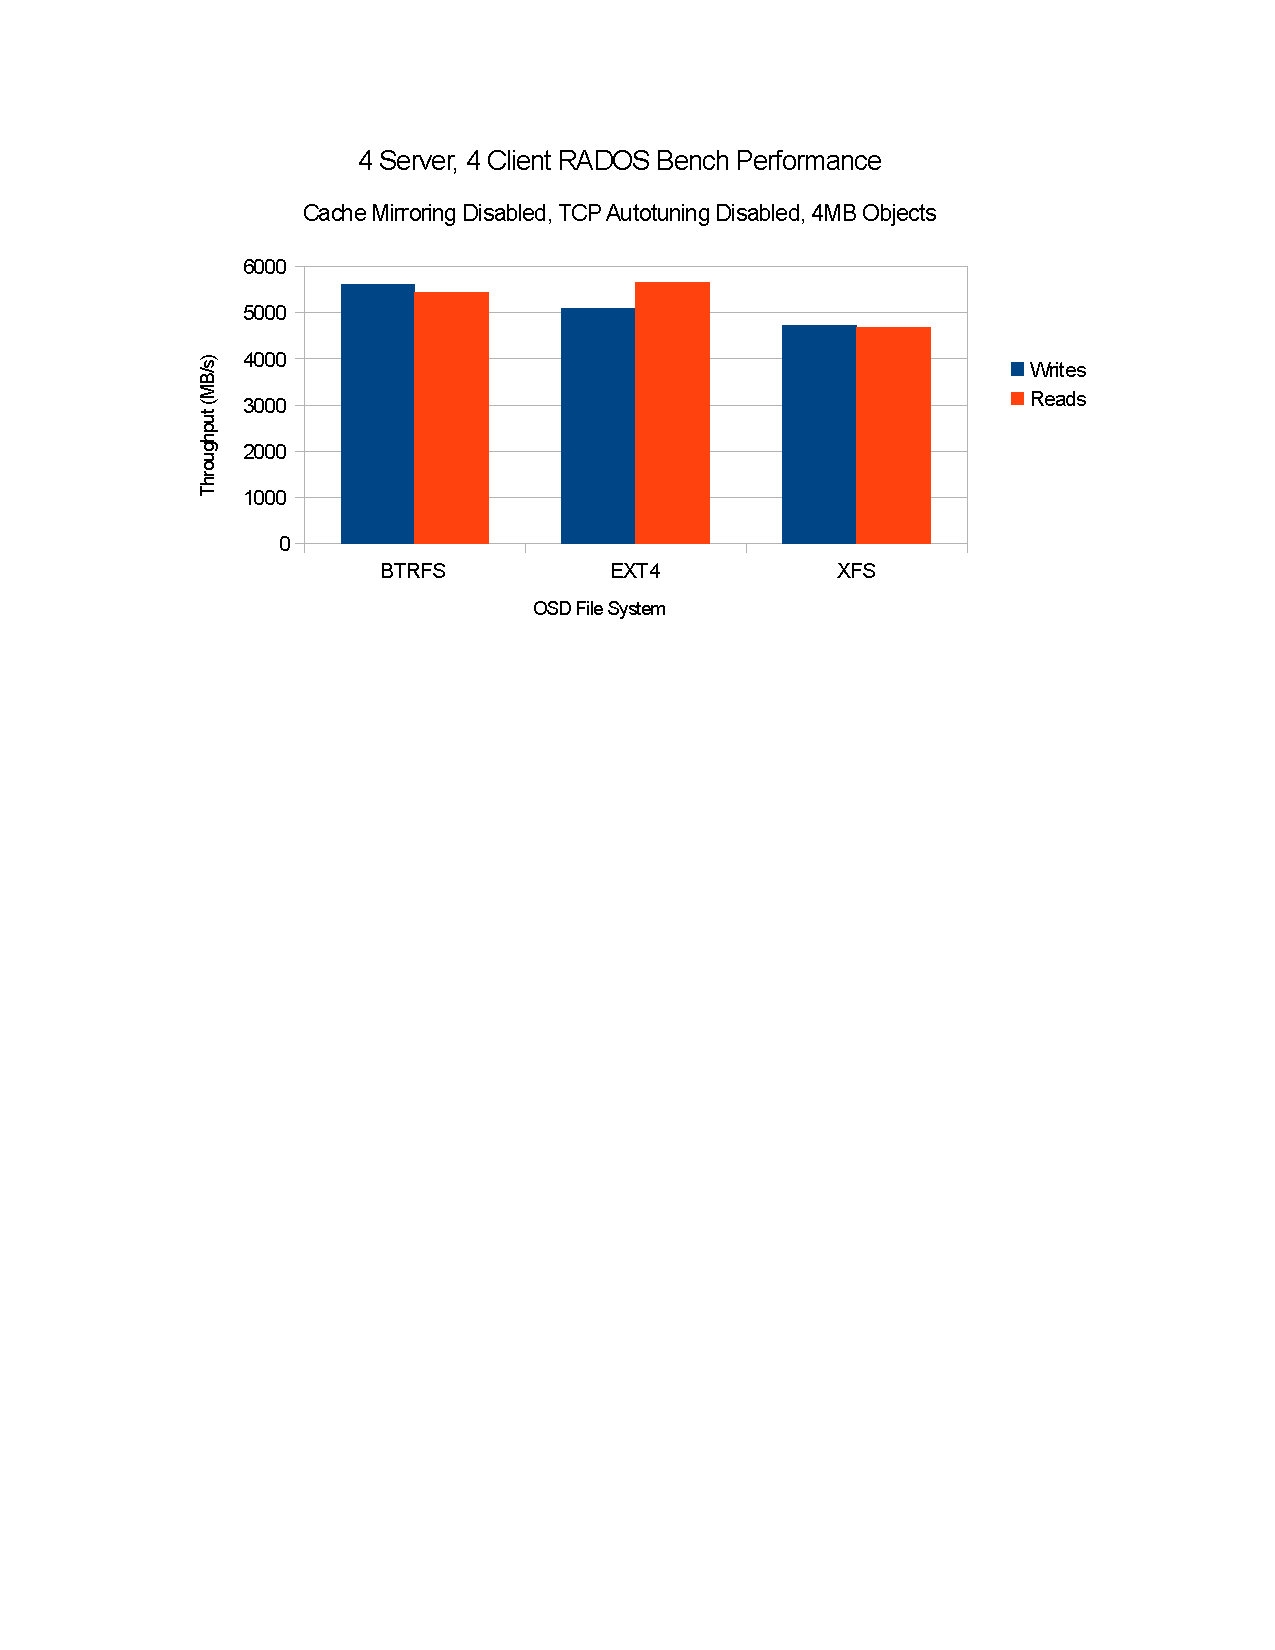
\includegraphics[width=3.5in]{rados-after-ddn-tcptune}
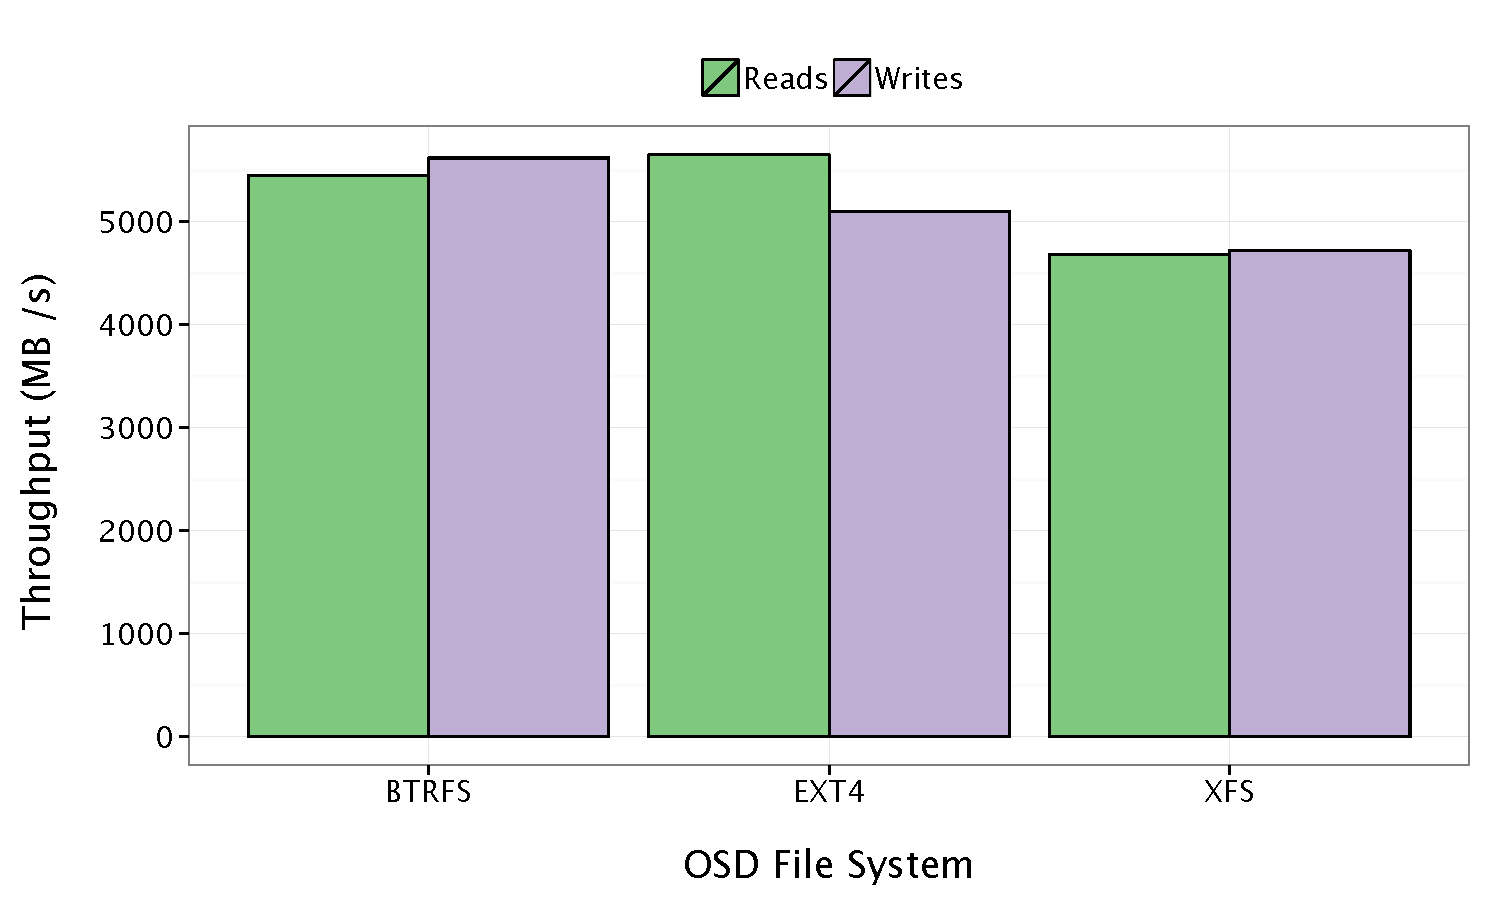
\includegraphics[width=3.5in]{autotune-disabled}
\caption{Evaluating RADOS bench with TCP auto tuning \textbf{disabled},  4 servers, 4
clients, 4 MB I/O}
\label{fig:rados-tcp-autotune-disabled}
\end{figure}


Luckily, the fix was fairly straightforward by setting system parameter
\url{/proc/sys/net/ipv4/tcp_moderate_rcvbuf} to zero on all nodes.  With this
change in place, We have observed this improving the performance significantly
on Ceph read operations. As shown in
Figure~\ref{fig:rados-tcp-autotune-disabled}.


%%%%%%%%%%%%%%%%%%%%%%%%%%%%% REMOVED for space

\begin{comment}

\begin{Verbatim}[fontsize=\small]
 echo 0 | sudo tee 
   /proc/sys/net/ipv4/tcp_moderate_rcvbuf
\end{Verbatim}

\end{comment}


Recent versions of Ceph work around this issue by manually controlling the TCP
buffer size.  

\subsubsection{Scaling on number of OSDs per server}

We also observed that using two or more client processes and many concurrent
operations are important when performing these tests.  We tested eight client
processes with 32 concurrent 4 MB objects in flight each. We created a pool
for each RADOS Bench process to ensure that object reads come from independent
pools (RADOS Bench is not smart enough to ensure that objects are not read by
multiple processes and thus possibly cached).  A sync and flush is performed
on every node before every test to ensure no data or metadata is in cache.
All tests were run with replication set to one. 

In the following test, a single Ceph host drives $n$ OSDs, where $n$ increases
from one to eleven. The result is illustrated in Figure~\ref{fig:osd-scale}.
We ran the test against a single client with four concurrent processes. In this
test case, we observe that the OSD server exhibits near linear scalability up to
nine OSDs, and is still trending upwards at eleven OSDs. This suggests that we
have not reached the saturation point yet. Additional testing would require
provisioning more OSDs on the SFA10K backend.


\begin{figure}[htb]
\centering
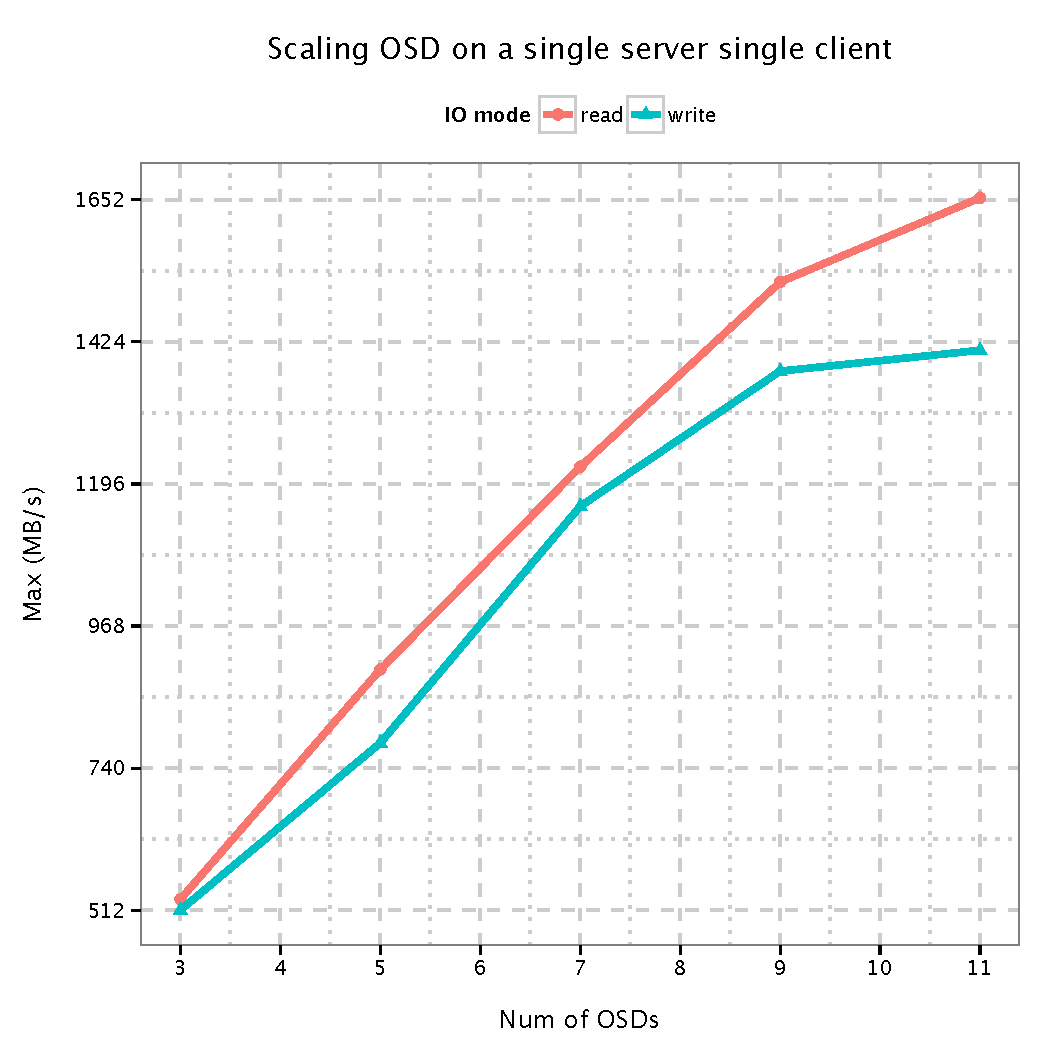
\includegraphics[width=3in]{data/rados_osd}
\caption{RADOS scaling on number of OSDs: single server single client}
\label{fig:osd-scale}
\end{figure}

\subsubsection{Scaling on number of OSD servers}

In this test, we exercise OSD servers from one to four, driven by four hosts
each with four RADOS Bench process. Each additional OSD server adds eleven
more OSDs into play.  Figure~\ref{fig:oss-scale} summarized the results.
Comparing to Figure~\ref{fig:rados-tcp-autotune-disabled}, the read
performance improved about 10\% given eight clients instead of four, but write
performance is mostly flat for reason explained below. We also observe that
Ceph exhibits linear scaling with regard to number of servers, at least in the
given number of servers.  However, the peak performance we are seeing is about
the half of what are expecting from the SFA10K (compare to the baseline block
I/O performance number presented in Section~\ref{sec:block-io}).

For writes, the lost performance is attributed to the way Ceph performs
journaling: Ceph does not support meta-data only journaling, therefore every
write is the equivalent of a double-write: once to the data device, once to
the journaling device. This effectively cuts the observed system bandwidth in
half. That said, it does not explain the read performance -- it is a little
better than write, but still far from the theoretical maximum.

\begin{figure}[htb]
\centering
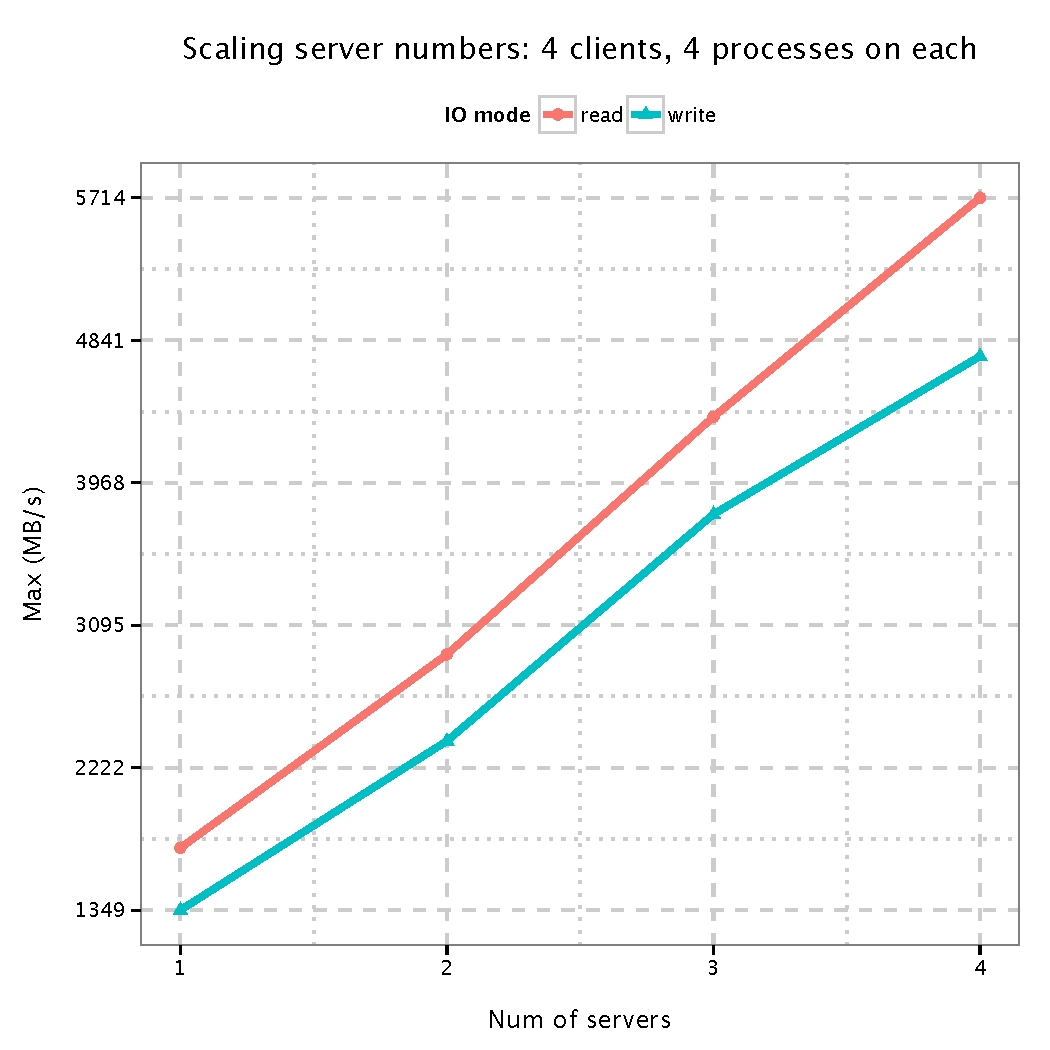
\includegraphics[width=3in]{data/rados_server}
\caption{RADOS scaling on number of servers, with 8 clients}
\label{fig:oss-scale}
\end{figure}

\subsection{Ceph File System Performance}
\label{sec:ior-initial}

\begin{figure*}[!t]

\centerline{\subfloat[4 KB transfer size]
{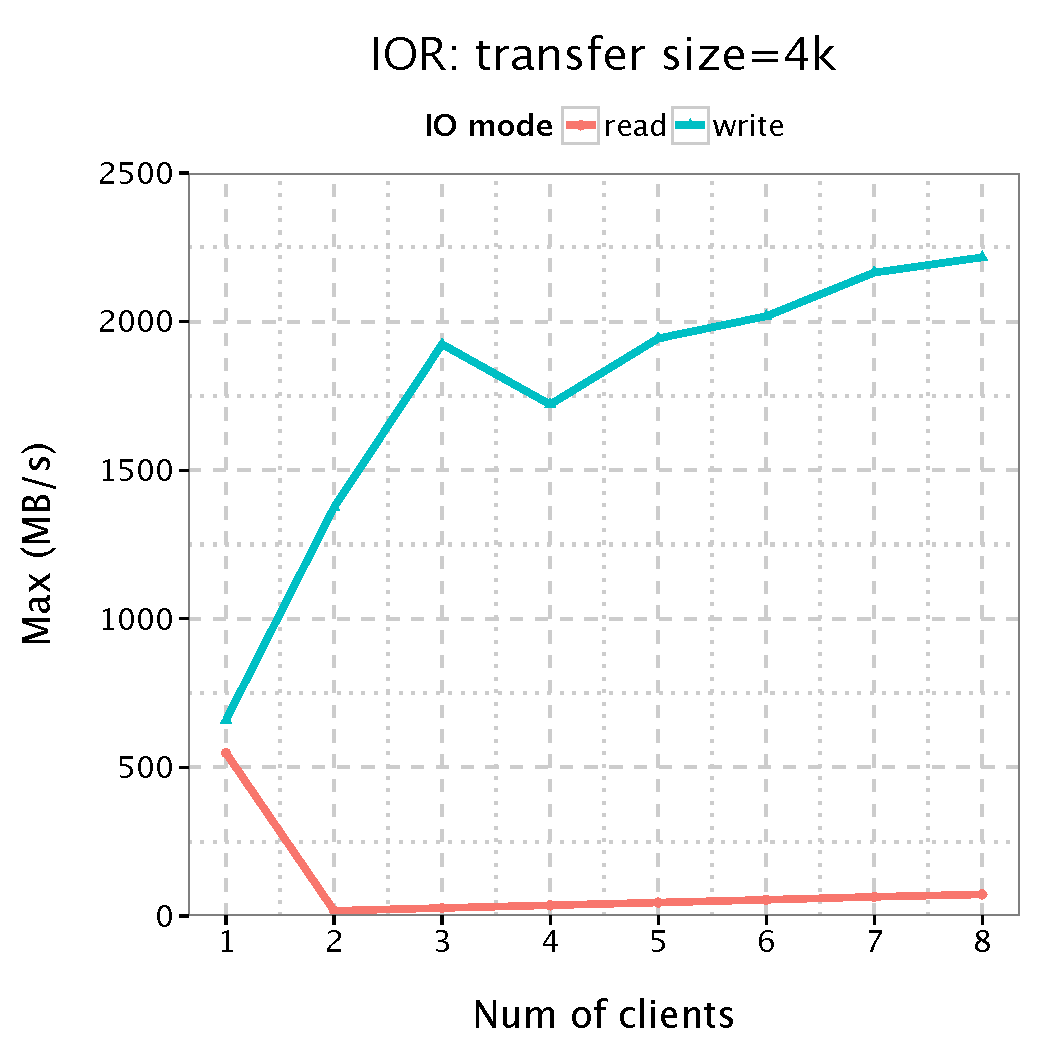
\includegraphics[width=3in]{data/ior_4k}
\label{fig:ior4k}}
\hfil
\subfloat[4 MB transfer size]
{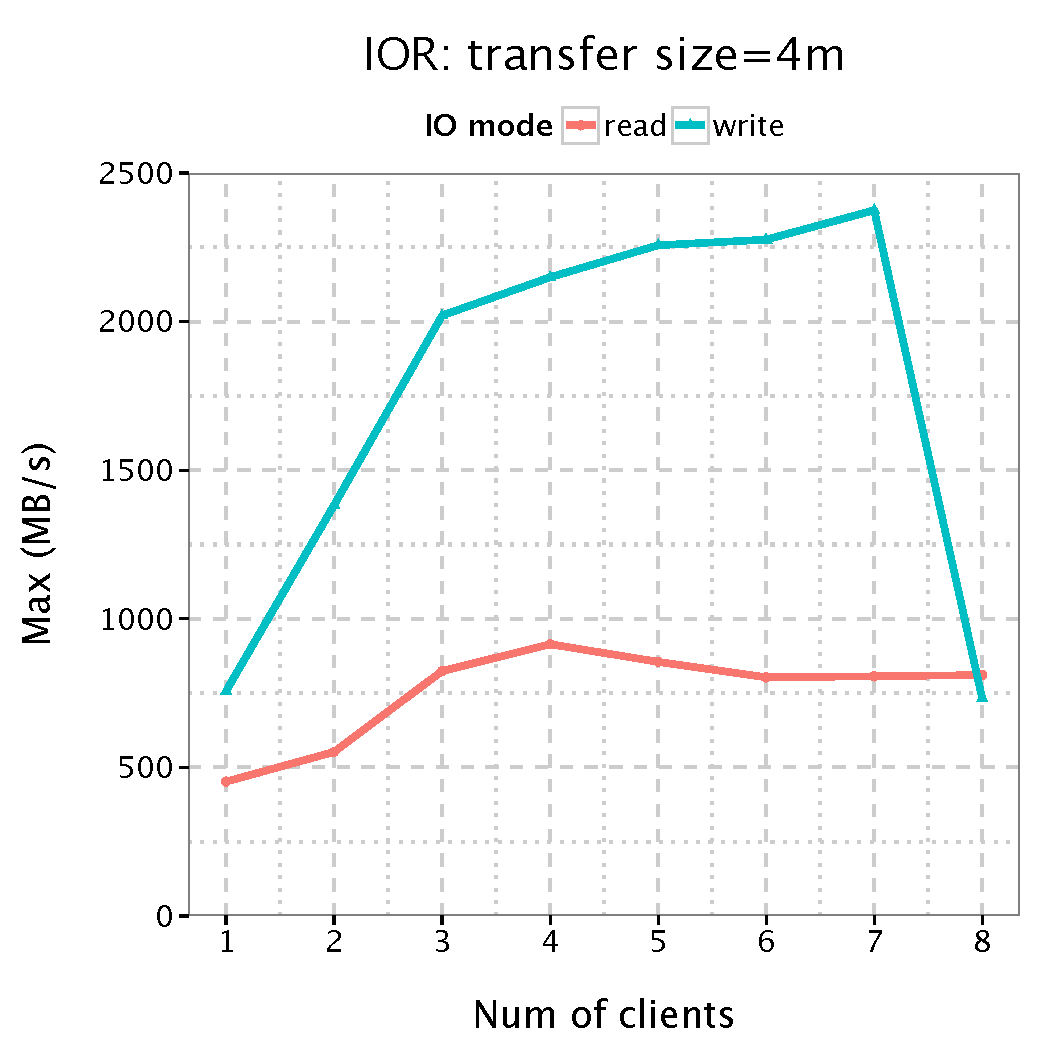
\includegraphics[width=3in]{data/ior_4m}
\label{fig:ior4m}}
}% end of centerline
\caption{CephFS scalability test with IOR}

\end{figure*}


We used the synthetic IOR benchmark
suite\cite{ior} for file system
level performance and scalability test.  
Each client node has 6 GB of physical memory, the block
size is set so as to mitigate cache effects. In addition, the test harness
program issues commands at the beginning of each test to free pagecache,
dentries and inodes.

%%%%%%%%%%%%%%%%%%%%%%%%%%%%%%%%%%%%%%%%%%%%
%%%%   COMMENT OUT IOR parameter table 
%%%%%%%%%%%%%%%%%%%%%%%%%%%%%%%%%%%%%%%%%%%%

\begin{comment}

\begin{table}[tb]
\caption{IOR parameter setup}
\label{tbl:ior}
\centering
\begin{tabular}{p{0.8in} | p{2in}}
    \hline
    IOR parameter & Note \\ \hline
    \verb!-F! & file per process \\ \hline
    \verb!-a POSIX! & use POSIX API \\ \hline
    \verb!-w -r -C! & do both write and read test, \verb!-C! is to change task
        ordering for read back so it will not read from the write cache. \\
        \hline
    \verb!-i 3 -d 5! & 3 iterations and delay 5 seconds betewen iterations \\ \hline  
    \verb!-e! & perform \verb!fsync()! upon POSIX write close \\ \hline
    \verb!-b 8g or 16g! & the block size \\ \hline
    \verb!-t 4k to 4m! & the transfer size \\ \hline
    \verb!-o file! & mandatory test file  \\    
    \hline
\end{tabular}
\end{table}


\begin{Verbatim}[fontsize=\small]
# sync
# echo 3 | tee /proc/sys/vm/drop_caches
\end{Verbatim}


Here, 0 is the default value of \verb!drop_caches!; 1 is to free pagecaches, 2
is to free dentries and inodes, 3 is to free pagecache, dentries, and inodes.

\end{comment}

Our initial tests was less than ideal as we encountered various issues.  The
full permutation of IOR parameters sweep were not explored due to I/O errors
we encountered.  We were, however, able to record results in two extreme cases
as far as transfer size is concerned: 4 KB and 4 MB, using a fixed number of
OSD servers (4) and fixed block size (8 GB), the results are illustrated in
Figure \ref{fig:ior4k} and \ref{fig:ior4m}, we make the following
observations:


\begin{itemize}

  \item The small read (4 KB transfer size) performance is almost an anomaly

  \item The large read (4 MB transfer size) performance is almost half of the
  RADOS read performance.
   
  \item The write performance is also about half of what we can obtain from
  RADOS Bench. When number of clients reaches 8, there is a significant
  performance drop, which is a poor sign for scalability. 

\end{itemize}

The bottom line is, though we have obtained decent performance number at RADOS
level, but it did not translate into file system-level performance. We will
investigate why it is so low compare to write performance and present improved
results in Section~\ref{sec:ceph-tuning}.


\subsection{Metadata Performance Evaluation}


In our particular setup, we only had one metadata server (MDS) configured.
Therefore, this is not a scalability test on the performance of Ceph clustered
MDS, which would have been very interesting.  Instead, we focus on a single MDS
performance and exercise it with up to 8 clients to observe the single MDS
performance scaling. We used
mdtest\footnote{\url{http://sourceforge.net/projects/mdtest/}} as our benchmark
tool. Mdtest parameters used for this test are:

\begin{itemize}
\item \verb!-w 1048576 -y!: for each created file, we write 1 MB data and
perform a sync operation.  This is a more realistic use case scenario than just
open, close and unlink sequence of metadata operations.

\item \verb!-n 1000!: Per client file \textit{and} directory workload. For
eight clients, the total number of files and directories in the workload is
8,000. Since we did not specify either \verb!-D! (indicates a directory only
workload) or \verb!-F! (indicates a file only workload), this is a mixture of
both directory and file workloads.

\item \verb!-d /mnt/cephfs/tmp!: we do specify a directory, but unlike under
Lustre file system, where you can have single client multiple mounts (for
increasing workload per client), here we just give the test an explicit home.

\item \verb!-u!: without this option, we are exercising shared directory; with
this option, we are exercising unique directories per test client processes.

\end{itemize}

Each test iterates five times and we are presenting the maximum out of all five iterations. 
We summarize the results as follows:

\begin{figure}[htb]
\centering
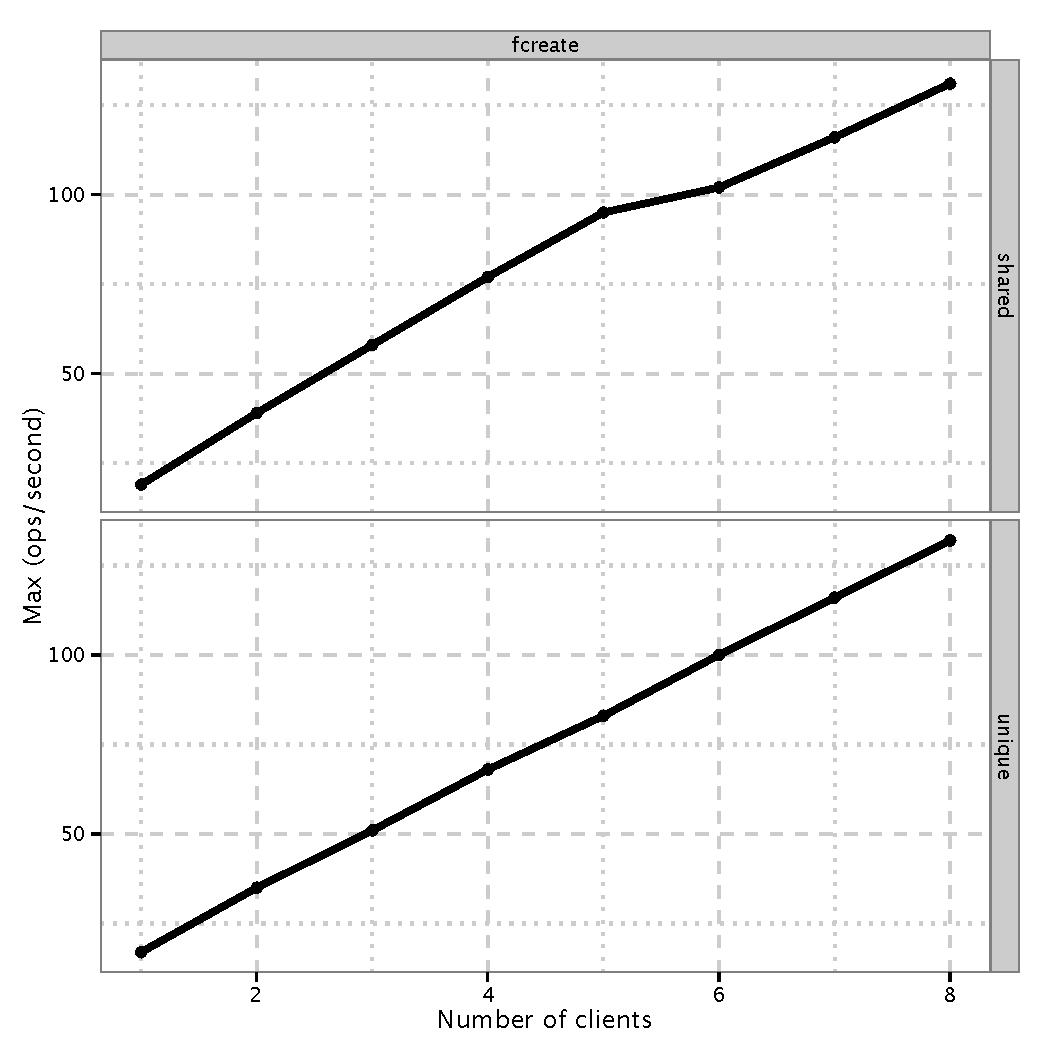
\includegraphics[width=3in]{data/mdtest-fcreate}
\caption{File creation vs.  number of clients}
\label{fig:mdtest-fcreate}
\end{figure}

\begin{figure}[htb]
\centering
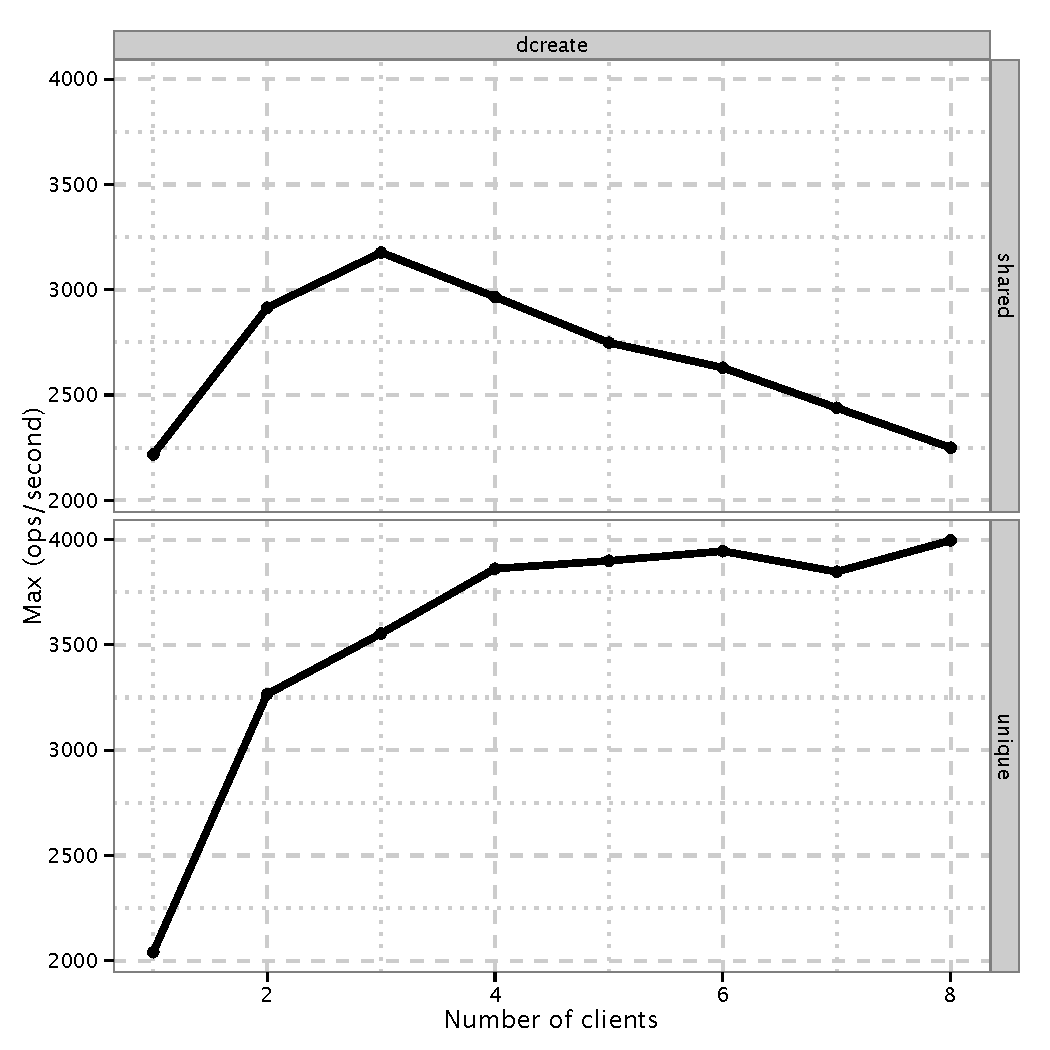
\includegraphics[width=3in]{data/mdtest-dcreate}
\caption{Directory creation vs. number of clients}
\label{fig:mdtest-dcreate}
\end{figure}


%Figure~\ref{fig:mdtest1c} is meant to give an overview on the trending of each
%directory (prefixed with d) and file (prefixed with f) operations, against the
%number of clients. Due to the scale difference, it doesn't convey the
%magnitude of lower numbers. 

\begin{itemize}

\item With either shared or unique directory (\verb!-u!), stat
operations for directories and files exhibit strong linear scaling. Same strong
linear scaling is also observed for file read operations. 

\item While the other operations seems unaffected or performance remains the
same by the number of clients, it is not so if we zoom in, see
figures \ref{fig:mdtest-fcreate} and \ref{fig:mdtest-dcreate}:  as number of clients
increases, we observed the contention for shared directory. The performance
degradation amount to 50\% or more.

\item Though the same saturation (or degradation) trend was not observed for
file creation operation, it is likely due to lack of workload stress on MDS.

\end{itemize}


The results also show that file creation rate is significantly lower than
directory creation rate. We stipulated two contributing factors: one is the file
creation is associated with 1 MB data write and followed by a fsync operation,
which is a rather heavy weight operation compare to directory creation. Another
factor is that we obtained above results while both RADOS and file
system-level performance are not tuned for optimal, yet. 

Next, we will describe the efforts and results on performance improvement at
both RADOS and file system-level. As consequence, we expect to see improved
metadata performance as well.


